\documentclass[../masters.tex]{subfiles}

\begin{document}
\graphicspath{{./imgs/}{../imgs/}} %look for images

\section{Linear Models}
In this section we consider probabilistic graphical models of the form shown in Figure \ref{fig_linmod}. This model is a generalisation of the graphical model seen in the Hidden Markov Model section. We now assume that the states ($X$) and observations ($Y$) are continuous random variables but the inputs ($U$) are deterministic. Models of this form are called Latent Linear Dynamical Systems (the famous Kalman Filter model falls into this category).
\begin{figure}[H] 
\centering
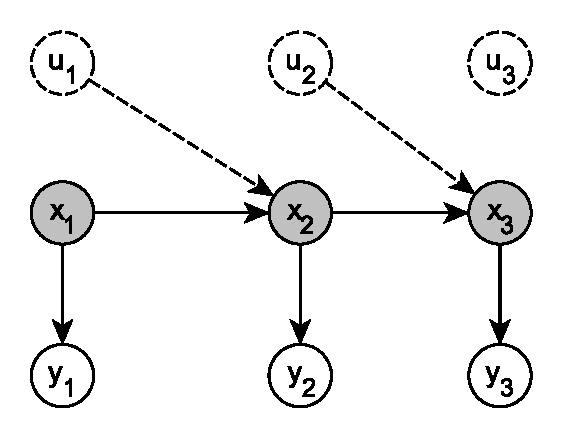
\includegraphics[scale=1.0]{linear_model.pdf}
\caption{Graphical model of this section}
\label{fig_linmod}
\end{figure}
In the previous section we developed inference algorithms but assumed that the transition and observation functions were discrete. We also noted that this assumption is not appropriate for continuous data. The reason is that one would invariably need to discretise the state domain and this would result in an intractably large state space if one requires reasonable resolution. To address this issue we extend the previous model to include both continuous states and observations. 

We assume linearity and that all the distributions are Gaussian. While these are strong assumptions they form the building blocks of much more expressive models as we will discover in the next section. 
%
%\bibliographystyle{plain}
%\bibliography{research}

\end{document}